% FindBack workshop paper draft.
% Build: latexmk -pdf findback.tex
%
% RULE FOR THIS FILE: no measured number is typed by hand. Every result is a macro
% from generated/results.tex, written by analysis/paper_figures.py from the phone logs.
% A macro with no data yet prints a red TBD.
\documentclass[sigconf,10pt]{acmart}
\settopmatter{printacmref=false}
\renewcommand\footnotetextcopyrightpermission[1]{}
\pagestyle{plain}

\usepackage{booktabs}
\usepackage{tikz}
\usetikzlibrary{arrows.meta,positioning,fit}

\newcommand{\TBD}{\textcolor{red}{TBD}}
\newcommand{\todo}[1]{\textcolor{red}{[#1]}}
\newcommand{\sys}{FindBack}
\InputIfFileExists{generated/results.tex}{}{}
% Fallbacks so the paper compiles before data exists.
% generated/results.tex (from analysis/paper_figures.py) is loaded first and wins.
% Anything defined here is NOT a measurement: it prints a red TBD, except the design
% constants in the last block, which are copied from the app's source.
\providecommand{\NSites}{\TBD}
\providecommand{\NRooms}{\TBD}
\providecommand{\NItems}{\TBD}
\providecommand{\NItemsPerSite}{\TBD}
\providecommand{\NQueriesPaired}{\TBD}
\providecommand{\NBenchCaptures}{\TBD}

\providecommand{\MarkerErrSessionMedianCm}{\TBD}
\providecommand{\MarkerErrMapMedianCm}{\TBD}
\providecommand{\MarkerErrMapPninetyCm}{\TBD}
\providecommand{\RelockJumpMedianCm}{\TBD}
\providecommand{\RelockJumpMedianDeg}{\TBD}

\providecommand{\VerifyAUC}{\TBD}
\providecommand{\ThresholdTau}{\TBD}
\providecommand{\VerifyTPRPct}{\TBD}
\providecommand{\VerifyFPRPct}{\TBD}
\providecommand{\LookalikeFPRThreshPct}{\TBD}
\providecommand{\LookalikeFPRMarginPct}{\TBD}

\providecommand{\WrongLeadMemoryPct}{\TBD}
\providecommand{\WrongLeadAlwaysPct}{\TBD}
\providecommand{\WrongLeadSelectivePct}{\TBD}
\providecommand{\LostRetrievalAlwaysPct}{\TBD}
\providecommand{\CapturesSelective}{\TBD}
\providecommand{\CaptureSavingPct}{\TBD}

\providecommand{\RegisterLatencyMs}{\TBD}
\providecommand{\VerifyLatencyMs}{\TBD}
\providecommand{\BytesPerItem}{\TBD}
\providecommand{\SecondsPerCapture}{\TBD}
\providecommand{\EnergyPerVerifymJ}{\TBD}

\providecommand{\FrameStalePct}{\TBD}
\providecommand{\FrameStaleAUC}{\TBD}
\providecommand{\ConfirmAtMarkerPct}{\TBD}
\providecommand{\ConfirmStalePct}{\TBD}
\providecommand{\CrossRoomNearPct}{\TBD}
\providecommand{\CrossRoomSecondsToNear}{\TBD}
\providecommand{\OnDeviceCaptures}{\TBD}
\providecommand{\WhatIfCapturesAucSeventy}{\TBD}
\providecommand{\WhatIfCapturesAucNinety}{\TBD}

% Design constants (from the app source, not measurements).
\providecommand{\RPresentCm}{30}
\providecommand{\FixAgreeSamples}{20}
\providecommand{\FixAgreeWindowS}{1.5}


\begin{document}

\title{Last Seen Is Not Where It Is: Selective Verification for On-Device Object Memory}

\author{Xiao Yan}
\affiliation{\institution{\todo{affiliation}}\country{USA}}
\author{\todo{co-authors}}
\affiliation{\institution{\todo{affiliation}}\country{USA}}

\begin{abstract}
Phones and glasses can now remember where a user put things and lead the user back.
What they store, however, is an observation from the past.
Presenting it as the item's current location is wrong whenever the item has moved or the device's
position in its own map has drifted, and the user walks to an empty spot.
Checking with a fresh camera capture on every query avoids this, but it costs the user a capture
each time, and visual matching makes its own mistakes.
We present \sys{}, a smartphone system that treats object memory as a historical claim.
It answers each query with one of three statements (\emph{last seen here}, \emph{seen here now},
or \emph{not confirmed}) and decides, from signals available before any new capture, whether a
fresh look is worth its cost.
\sys{} runs entirely on the device and needs no markers: it keeps its own lightweight map,
re-attached in each session from a single fix point, with a graph of walked paths for
room-level guidance.
In \NSites{} homes with \NItems{} items and \NQueriesPaired{} paired queries, memory alone gave a
wrong lead in \WrongLeadMemoryPct{}\% of queries.
Selective verification reduced this to \WrongLeadSelectivePct{}\% with \CapturesSelective{}
captures per query, \CaptureSavingPct{}\% fewer than always verifying.
\end{abstract}

\maketitle

% ---------------------------------------------------------------------------
\section{Introduction}

``Where did I put my keys?'' is one of the oldest requests made of a memory aid.
Mobile devices can now answer it without tags on the objects: a phone or a pair of glasses sees
an item, stores its appearance and its position in a spatial map, and later points the user back
to it \todo{cite: object finders, episodic memory}.
Persistent augmented-reality frameworks make the spatial half of this practical on commodity
phones.

The stored position, however, is a fact about the past.
Between the moment an item was remembered and the moment the user asks for it, two things can go
wrong.
The \emph{world} can change: somebody moves the item.
The \emph{frame} can change: the device's estimate of where it is in its own map drifts as the
user walks, or is re-established imperfectly after a restart.
In both cases a system that draws a confident marker at the stored position sends the user to the
wrong place.
We call this a \emph{wrong lead}.
It costs more than the walk.
A user who has been misled a few times stops trusting the marker when it is right
\todo{cite: automation bias}.

The obvious remedy is to look again: ask the user to aim the camera at the remembered spot and
match the fresh view against the stored appearance.
Doing this on every query has three costs.
The user must walk to the spot, aim, and wait, even when the item has plainly not moved.
Each capture costs computation and energy.
And matching is imperfect: it can confirm a look-alike, or fail to confirm an item that is there.
A system that always verifies trades wrong leads for extra effort and a new kind of error.

This paper argues for a middle path.
A stored location should be presented as what it is, a historical claim, and the system should
choose \emph{per query} whether a fresh look is worth its cost.
The choice has to be made from signals that are available \emph{before} any new capture,
otherwise it costs as much as verifying.
Such signals exist.
How old is the memory?
Does this item tend to move?
How far has the phone walked, and has tracking been interrupted, since its map was last fixed to
the world?

We make three contributions.

\begin{itemize}
\item \textbf{A formulation.} We define the object-memory query as a three-way answer
  (\emph{last seen here}, \emph{seen here now}, \emph{not confirmed}) and evaluate a policy by the
  wrong leads it produces against the captures it requests (\S\ref{sec:problem}).
\item \textbf{A system.} \sys{} is an on-device Android system built on ARCore.
  It keeps a marker-free persistent map of a home, guides the user along paths they have walked,
  verifies with a fresh capture, and logs everything needed to replay each query under any
  capture policy (\S\ref{sec:design}).
\item \textbf{An evaluation} in \NSites{} homes that measures localization error across rooms and
  restarts, verification accuracy against absent items and look-alikes, and the trade-off between
  wrong leads and captures for memory-only, always-verify and selective policies
  (\S\ref{sec:eval}).
\end{itemize}

% ---------------------------------------------------------------------------
\section{Problem}
\label{sec:problem}

\paragraph{Setting.}
A user \emph{registers} an item by pointing the phone at it and confirming a name.
The system stores a \emph{record}: an appearance embedding of the item, its position in a
persistent map, the room, and the time.
Later the user issues a \emph{query} for the item by name.
The system may answer from the record alone, or first request one \emph{capture}: the user aims the
camera at the remembered spot and the system compares what it sees with the record.
We limit a query to one capture, the most a user will tolerate for a routine request.

\paragraph{Answers.}
\sys{} gives one of three answers.
\emph{Last seen here} is the record, labelled as history.
\emph{Seen here now} means a capture matched the record.
\emph{Not confirmed} means a capture did not match.
The system never says that an item has moved: a failed match can also come from a poor view or
from drift, and the system cannot tell these apart.

\paragraph{Outcomes.}
After each query the experimenter records where the item really is.
An answer of \emph{last seen here} or \emph{seen here now} is a \emph{correct lead} if the item is
at the marked position, within \RPresentCm{}\,cm, and a \emph{wrong lead} otherwise.
An answer of \emph{not confirmed} is a \emph{correct warning} if the item is not there, and a
\emph{lost retrieval} if it is.
Wrong leads are the error this paper targets.
Lost retrievals are the price of verification errors.

\paragraph{Why memory goes stale.}
A wrong lead has two independent causes.
With \emph{world staleness}, the item is no longer where it was.
With \emph{frame staleness}, the item has not moved but the marker is drawn in the wrong place,
because the device's map is misaligned with the world.
The two call for different signals, and a policy that watches only one of them is blind to the
other.

\paragraph{Policies.}
A policy maps the \emph{pre-capture signals} of a query to a decision: capture or not.
\emph{Memory-only} never captures.
\emph{Always-verify} always does.
A \emph{selective} policy captures when an estimate of the risk that the record is stale exceeds a
threshold.
Sweeping that threshold traces a curve from memory-only to always-verify.
The question is how far below the straight line between them the curve lies, that is, how much
better than capturing at random the signals let us do.

% ---------------------------------------------------------------------------
\section{Design}
\label{sec:design}

\begin{figure}[t]
\centering
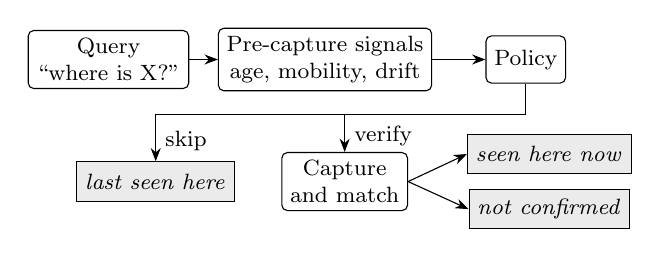
\begin{tikzpicture}[
  font=\footnotesize, >=Stealth,
  box/.style={draw, rounded corners=2pt, align=center, inner sep=3pt, minimum height=6mm},
  ans/.style={draw, align=center, inner sep=3pt, minimum height=5mm, fill=black!8}]
\node[box] (q)   at (0,0)    {Query\\``where is X?''};
\node[box] (sig) at (2.75,0) {Pre-capture signals\\age, mobility, drift};
\node[box] (pol) at (5.3,0)  {Policy};
\node[ans] (last) at (0.6,-1.55) {\emph{last seen here}};
\node[box] (cap)  at (3.0,-1.55) {Capture\\and match};
\node[ans] (now)  at (5.6,-1.2)  {\emph{seen here now}};
\node[ans] (not)  at (5.6,-1.9)  {\emph{not confirmed}};
\draw[->] (q) -- (sig);
\draw[->] (sig) -- (pol);
\coordinate (split) at (5.3,-0.7);
\draw (pol.south) -- (split);
\draw[->] (split) -| node[pos=0.78, right] {verify} (cap.north);
\draw[->] (split) -| node[pos=0.78, right] {skip} (last.north);
\draw[->] (cap.east) -- (now.west);
\draw[->] (cap.east) -- (not.west);
\end{tikzpicture}
\caption{A query in \sys{}. The policy sees only signals that exist before any new capture.}
\label{fig:overview}
\end{figure}

Figure~\ref{fig:overview} shows a query.
This section describes the four parts that make it work: a persistent map that needs no markers,
guidance that respects walls, verification, and the capture policy.

\subsection{A home map from one fix point}

ARCore tracks the phone's motion within a session but offers no way to save its map to local
storage; its persistent anchors are hosted by a cloud service.
An earlier version of \sys{} stored positions relative to a printed reference picture in each
room.
That needs one picture per room, and it failed in practice for a simple reason: users cannot be
expected to print and hang markers.

\sys{} instead keeps its own map and re-attaches it in each session from \emph{one} known point.
The map frame and ARCore's session frame are both aligned with gravity, so they differ only by a
rotation about the vertical axis and a translation: four degrees of freedom, not six.
\sys{} never uses a full six-degree transform between them.
The reason is error amplification.
A fix point observed with a small tilt error would, under a six-degree transform, lift or sink
every remembered position in proportion to its distance, and far rooms would suffer most.
With gravity fixed by the inertial sensors, only the heading error remains: a 2$^\circ$ error
moves a point 5\,m away by 17\,cm, and by nothing vertically.

A \emph{fix point} is anything the phone can observe again to recover those four numbers.
\sys{} supports two kinds.
A \emph{picture} is a known image, shown on a tablet or printed, that ARCore's image tracking can
detect; \sys{} averages its pose until \FixAgreeSamples{} samples within \FixAgreeWindowS{}\,s
agree to within 2\,cm and 2$^\circ$, and accepts samples only when the camera is close enough for
the image to be well resolved.
A \emph{spot} needs no object at all: the user rests the phone in a pose they can repeat, such as
against a door frame, and presses a button.
To help the user repeat the pose, \sys{} overlays a faint image of the saved view on the live
camera.
The heading of a spot is taken from whichever screen axis is closer to horizontal, so the phone
may stand upright or lie on its side.
After a fix, an ARCore anchor carries the fix pose, so that ARCore's own corrections to its map
move the home map with it.
Further fix points can be added in other rooms and act as checkpoints.

Each fix resets three \emph{drift proxies}: the distance the camera has travelled since the fix,
the number of tracking interruptions of one second or more, and the elapsed time.
They cost nothing to maintain and are the policy's view of frame staleness.

\subsection{Guidance that respects walls}

A marker at the remembered position is enough when the user is standing next to it.
From another room it is worse than useless: an arrow pointing straight at the item points through
a wall, says nothing about which room to go to, and is wrong as soon as the frame has drifted.

While the map is located, \sys{} records where the phone goes as a \emph{walk graph}: a node every
half metre, with an edge between two nodes only if the phone moved directly from one to the
other.
Every edge is therefore a path somebody has walked.
The user names rooms as they enter them, and the nodes they visit take that label; later, walking
onto labelled nodes tells \sys{} which room the user is in.
Each record also stores where the user \emph{stood} when registering the item, a walkable point
next to it.

Guidance then depends on where the user is.
Far from the item, \sys{} names the room and shows the shortest walked route to the standing
point, with an arrow to a waypoint a short distance ahead along the route.
Only when the remaining route is short, or the user is known to be in the item's room, does it
show a ring on the item itself.
If the map has not been located in this session, \sys{} shows the item's photograph and room and
asks the user to visit a fix point; it shows no arrow at all.

\subsection{Memory and verification}

\paragraph{Registration.}
The user taps the item on screen.
\sys{} finds the tapped surface point from ARCore's depth and plane estimates and rejects
implausible depths.
An on-device object detector proposes boxes; \sys{} keeps the smallest box that contains the tap
and has a plausible physical size, and otherwise crops a fixed physical window around the tapped
point, sized from the camera intrinsics and the depth.
The crop is embedded with a compact image model, and the record stores the embedding, the position
in the map frame, the standing point, the room, and how often the user expects the item to move.
The user's name for the item and the detector's raw label are stored separately.

\paragraph{Verification.}
For a capture, \sys{} projects the remembered position into the current camera frame and crops
the same physical window, rescaled for the new distance.
Because the projection is only as good as the frame, it also considers detector boxes that
overlap the window and have a similar size.
Each candidate is embedded and compared with the record by cosine similarity.
The capture confirms the item if the best similarity reaches a threshold $\tau$.
We also evaluate a stricter rule that additionally requires the best candidate to match the
queried record better than any other stored record by a margin, which targets look-alikes.

\paragraph{Records are snapshots.}
A confirmed capture does not rewrite the record.
A record changes only when the user tells \sys{} that an item has a new place, which creates a
new record linked to the old one.
This keeps the meaning of ``age'' simple (time since the user last vouched for the position) and
gives each item a history of moves.

\subsection{Deciding when to look}

The policy may use only what is known before a capture.

\begin{itemize}
\item \emph{World staleness:} the age of the record; the user's estimate of how often the item
  moves; how many times the item has been moved before.
\item \emph{Frame staleness:} whether the position comes from an anchor created in this session or
  from the home map; the drift proxies; the kind of fix point.
\end{itemize}

Similarity to other stored items is deliberately not a trigger.
A look-alike does not make the record more likely to be stale.
It makes a \emph{capture} less trustworthy, so it belongs in the matching rule, as the margin test
above.

\sys{} ships with a simple rule: verify when the record is older than a limit, or when the
position comes from the map and the phone has walked far or lost tracking since the last fix.
For the evaluation we also fit a logistic model of the probability that a lead is wrong given the
signals, and verify when that probability exceeds a threshold $\theta$.
If a wrong lead costs the user $c_w$ and a capture costs $c_c$, capturing is worthwhile when the
estimated probability exceeds roughly $c_c/c_w$; sweeping $\theta$ covers every such trade-off.

% ---------------------------------------------------------------------------
\section{Implementation}

\sys{} is an Android application in Kotlin for the Google Pixel~8, built on ARCore~1.48 with the
Depth and Augmented Images APIs.
It uses ML~Kit's on-device object detector for class-agnostic boxes and a MobileNet-V3 image
embedder (1024 dimensions) through MediaPipe.
Nothing leaves the phone: there is no cloud anchor, no remote inference, and no account.
A record takes about \BytesPerItem{}\,bytes including its photograph.

\paragraph{Instrumentation for policy replay.}
Comparing policies fairly requires the same queries under each policy.
Running each condition live would let the world change between conditions.
\sys{} instead logs, for every query, the pre-capture signals at the moment the query starts, one
capture with the similarity of every candidate and their embeddings, and the ground truth entered
by the experimenter.
Any policy and any matching threshold can then be replayed offline on identical data.
Thresholds are chosen on development sessions and frozen before test sessions.

% ---------------------------------------------------------------------------
\section{Evaluation}
\label{sec:eval}

We ask four questions.
(1) How accurately does a home map re-attached from one fix point place markers across rooms and
restarts?
(2) How well does on-device matching tell an item from an empty spot, another object, or a
look-alike?
(3) How many captures does a selective policy need to avoid the wrong leads of memory alone?
(4) What does the system cost in time, storage and energy?

\subsection{Setup}

\InputIfFileExists{generated/table_dataset.tex}{}{%
\begin{table}[t]
\caption{Dataset. \todo{generated by analysis/paper\_figures.py}}
\label{tab:dataset}
\centering\small
\begin{tabular}{lr}
\toprule
Homes / rooms & \NSites{} / \NRooms{} \\
Items & \NItems{} \\
Paired queries & \NQueriesPaired{} \\
Labelled benchmark captures & \NBenchCaptures{} \\
\bottomrule
\end{tabular}
\end{table}}

We collected data in \NSites{} homes with \NRooms{} rooms in total.
Table~\ref{tab:dataset} summarizes it.
The experimenters were the authors.
All sessions used a Pixel~8.

\paragraph{Localization (E1).}
In each home we set a home fix point, walked through the rooms, and registered \NItemsPerSite{}
items.
We then restarted the application three times; after each restart we located the map again and,
for every item, tapped its true centre on screen to measure the distance from the marker.

\paragraph{Verification benchmark (E2).}
For each item we took captures with the item in place from near, far and oblique viewpoints and
under different lighting, with the item removed, with a different object in its place, and, where
one was available, with a look-alike.
Each capture was labelled on the phone as it was taken.

\paragraph{Controlled trials (E3).}
Before each round a script chose, at random and independently of every signal the policy uses,
what to do with each item: leave it, remove it, move it nearby, or put another object in its
place.
The experimenter applied the changes and then queried every item once, capturing exactly once per
query.
Because the changes are scripted, E3 measures what each policy does when memory is stale and what
it costs; it says nothing about how often memory is stale in daily life.

\paragraph{Deployment (E5).}
To measure that, \todo{two} of the authors used \sys{} at home for \todo{five} days.
They lived normally, queried every item twice a day, and told \sys{} when they found an item
somewhere else.
Here items move for their own reasons, and the signals can only help if they really predict it.

\subsection{Localization across rooms and restarts}

\todo{Figure F1: CDF of marker error by position source and by room; error against metres walked.}
With the position taken from a same-session anchor, the median marker error was
\MarkerErrSessionMedianCm{}\,cm.
After a restart, with the map re-attached from one fix point, it was \MarkerErrMapMedianCm{}\,cm
(90th percentile \MarkerErrMapPninetyCm{}\,cm).
\sys{} named the item's room correctly in \RoomCorrectPct{}\% of queries.
Locking twice onto the same spot moved the map by a median of \RelockJumpMedianCm{}\,cm and
\RelockJumpMedianDeg{}$^\circ$.

\subsection{Verification accuracy}

\todo{Figure F2: ROC by negative type; true-positive rate by viewing condition.}
On \NBenchCaptures{} labelled captures, matching reached an AUC of \VerifyAUC{}.
At the threshold chosen on the development split ($\tau=\ThresholdTau{}$) it confirmed
\VerifyTPRPct{}\% of items that were present and falsely confirmed \VerifyFPRPct{}\% of the
others.
Look-alikes were falsely confirmed in \LookalikeFPRThreshPct{}\% of captures with the threshold
alone and \LookalikeFPRMarginPct{}\% with the margin rule.

\subsection{Wrong leads against captures}

\todo{Figure F3: captures per query against wrong-lead rate for all policies; E3 and E5 panels.}
Across \NQueriesPaired{} paired queries, memory alone gave a wrong lead in
\WrongLeadMemoryPct{}\% of them.
Always verifying reduced this to \WrongLeadAlwaysPct{}\%, at one capture per query, and lost
\LostRetrievalAlwaysPct{}\% of retrievals to failed matches.
The selective policy gave \WrongLeadSelectivePct{}\% wrong leads with \CapturesSelective{}
captures per query.
\todo{Compare with the random-capture line and the oracle; report the signal ablation; report E3
and E5 separately.}

\subsection{Cost}

\todo{Table T2.}
Registering an item took \RegisterLatencyMs{}\,ms of processing and a verification
\VerifyLatencyMs{}\,ms.
From reaching the item to seeing the result, a capture took the user \SecondsPerCapture{}\,s.
A verification consumed \EnergyPerVerifymJ{}\,mJ above tracking alone.

% ---------------------------------------------------------------------------
\section{Discussion and Limitations}

\paragraph{The signals must earn their place.}
A selective policy helps only if its signals predict staleness.
In scripted trials we choose what moves, so those trials cannot show this; only the deployment
can.
\todo{State the outcome honestly once E5 is analysed, including if the signals do not help.}

\paragraph{One floor, one device.}
The map treats the home as a single floor, and all data come from one phone model.
Heading error at the fix point grows into position error with distance; in large homes, more fix
points are the remedy.

\paragraph{Appearance matching is the weak link.}
A compact embedding of a small crop is sensitive to viewpoint and lighting.
A stronger model would raise the ceiling for always-verify and narrow the case for skipping
captures; a weaker one does the opposite.
The framework is the same.

\paragraph{The user is the sensor.}
\sys{} learns about an item only when the user registers it, verifies it, or reports a move.
Glasses that observe continuously would change which signals are available, and would make
``capture'' nearly free; the same accounting of wrong leads against sensing cost still applies.

% ---------------------------------------------------------------------------
\section{Related Work}

\todo{Written from paper/research/related\_work.md once the references are verified.}

% ---------------------------------------------------------------------------
\section{Conclusion}

A remembered location is a statement about the past.
\sys{} presents it as one, and spends a fresh look only where the evidence suggests the past may
no longer hold.
\todo{One sentence with the headline number once measured.}

\begin{acks}
\todo{Generative-AI disclosure, as the venue requires.}
\end{acks}

\bibliographystyle{ACM-Reference-Format}
\bibliography{refs}

\end{document}
